\documentclass{beamer}
\beamertemplatenavigationsymbolsempty
\usepackage[french]{babel}
\usepackage{fontspec}
\usepackage{amsmath, amsthm, amsfonts}
\usepackage[separate-uncertainty]{siunitx}
\usepackage{xcolor}
\usepackage{tikz}
\usepackage{tikz-cd}
\usepackage[object=vectorian]{pgfornament}
\usepackage{circuitikz}
\usepackage{hyperref}
\usepackage{caption}
\usepackage{booktabs}
\usepackage{mathtools}
\usepackage{longtable}
\usepackage[version=3]{mhchem}
\usepackage{marginnote}
\usepackage[framemethod=tikz]{mdframed}


% Paul Tol's qualitative palette
% ``bright''.https://personal.sron.nl/~pault/#sec:qualitative
\definecolor{tblue}{HTML}{4477AA}
\definecolor{tcyan}{HTML}{66CCEE}
\definecolor{tgreen}{HTML}{228833}
\definecolor{tyellow}{HTML}{CCBB44}
\definecolor{tred}{HTML}{EE6677}
\definecolor{tpurple}{HTML}{AA3377}
\definecolor{tgrey}{HTML}{BBBBBB}


% Justification for marginnotes.
\renewcommand*{\raggedleftmarginnote}{}
\renewcommand*{\raggedrightmarginnote}{}


% Styles for mdframed environments.
\newmdenv[backgroundcolor=tgreen!10,linecolor=tgreen!30]{reponsebox}
\newmdenv[backgroundcolor=tyellow!10,linecolor=tyellow!30]{diapobox}
\newmdenv[backgroundcolor=tred!10,linecolor=tred!30]{fondamentalbox}

% Default arrow for tikz and style for positive and negative objects.
\tikzset{>=latex,
    negative/.style={draw=teal!70!black, fill=teal!10, thick},
    positive/.style={draw=red, fill=red!10, thick}}
\usetikzlibrary{matrix,calc,decorations.pathreplacing,decorations.pathmorphing,decorations.markings}

% French locale for numbers and negative exponent for units.
\sisetup{locale=FR, per-mode=symbol}

\newcommand{\abs}[1]{\left| #1 \right|}
\newcommand{\rhat}{\vec{\hat{r}}}
\newcommand{\xhat}{\vec{\imath}}
\newcommand{\yhat}{\vec{\jmath}}
\newcommand{\zhat}{\vec{k}}
\newcommand{\real}{\mathbb{R}}
\newcommand{\der}[2]{\frac{\mathrm{d}#1}{\mathrm{d}#2}}
\newcommand{\pder}[2]{\frac{\partial\ #1}{\partial\ #2}}
\newcommand{\dif}{\mathrm{d}}
\newcommand{\ddif}{\,\mathrm{d}}
\newcommand{\grad}{\vec{\nabla}}
\newcommand{\exemple}[1]{\begin{fullwidth}#1\end{fullwidth}}
\newcommand{\norm}[1]{\lVert\ #1\ \rVert}
\newcommand{\vu}{\vec{u}}
\newcommand{\vv}{\vec{v}}
\newcommand{\vr}{\vec{r}}
\newcommand{\va}{\vec{a}}
\newcommand{\vF}{\vec{F}}
\newcommand{\vE}{\vec{E}}
\newcommand{\vB}{\vec{B}}
\newcommand{\vecxyz}[3]{#1 \xhat\ + #2 \yhat\ + #3 \zhat}
\newcommand{\vecxy}[2]{#1 \xhat\ + #2 \yhat}
\newcommand{\coulombcst}{k}
\newcommand{\emf}{\ensuremath{\mathcal{E}}}
\newcommand{\eval}{\SI{1.602e-19}{C}}
\newcommand{\kval}{\SI{8.99e9}{Nm^2 \per C^2}}

% Nice separator line
\newcommand{\sectionline}{
    \noindent
    \begin{center}
        \resizebox{0.5\linewidth}{1ex}
    {{%
    {\begin{tikzpicture}
    \node  (C) at (0,0) {};
    \node (D) at (9,0) {};
    \path (C) to [ornament=85] (D);
    \end{tikzpicture}}}}
    \end{center}
}

\theoremstyle{definition}
\newtheorem*{defn}{Definition}


\usepackage[version=3]{mhchem}

\setbeamercolor{title}{fg=tblue}
\setbeamercolor{frametitle}{fg=tblue}
\setbeamercolor{structure}{fg=tblue}

% Make footnotesize smaller
\makeatletter
\renewcommand\footnotesize{%
   \@setfontsize\footnotesize\@viipt{11}%
   \abovedisplayskip 8\p@ \@plus2\p@ \@minus4\p@
   \abovedisplayshortskip \z@ \@plus\p@
   \belowdisplayshortskip 4\p@ \@plus2\p@ \@minus2\p@
   \def\@listi{\leftmargin\leftmargini
               \topsep 4\p@ \@plus2\p@ \@minus2\p@
               \parsep 2\p@ \@plus\p@ \@minus\p@
               \itemsep \parsep}%
   \belowdisplayskip \abovedisplayskip
}
\makeatother

\title{Électricité et magnétisme}
\subtitle{Chapitre 5 - Potentiel électrique}
\date{29 septembre 2021}
\author{Loïc Séguin-Charbonneau}
\institute{Cégep Édouard-Montpetit}

\begin{document}

\maketitle


\begin{frame}{Deux grandes plaques parallèles}

On considère deux grandes plaques parallèles connectées à une source de
tension. Chacune des plaques a une surface $A$. Si on applique une différence
de potentiel $\Delta V$ entre les deux plaques, quelle charge sera emmagasinée
sur chacune des plaques?

\begin{center}
  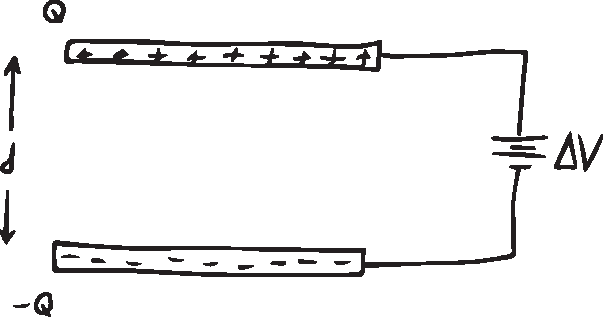
\includegraphics[scale=0.4]{../figures/condensateur-plan.pdf}
\end{center}

\end{frame}


\begin{frame}[t]{Deux grande plaques parallèles}

On considère deux grandes plaques parallèles connectées à une source de
tension. Chacune des plaques a une surface $A$. Si on applique une différence
de potentiel $\Delta V$ entre les deux plaques.

\begin{center}
  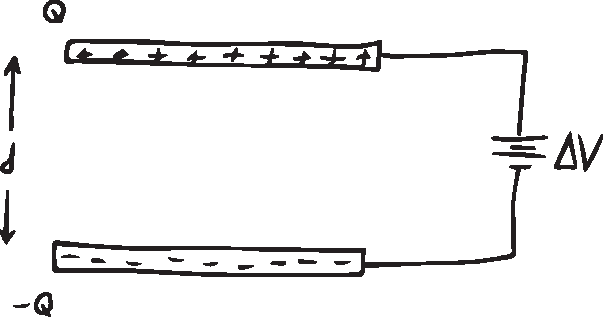
\includegraphics[scale=0.4]{../figures/condensateur-plan.pdf}
\end{center}


\only<1-2>{
  Quelle expression décrit le champ électrique entre les plaques?

  \begin{enumerate}[A.]
    \item $\vE = \frac{\sigma}{\varepsilon_0}$ vers le haut
    \item<alert@2> $\vE = \frac{\sigma}{\varepsilon_0}$ vers le bas
    \item $\vE = \frac{\sigma}{2\varepsilon_0}$ vers le haut
    \item $\vE = \frac{\sigma}{2\varepsilon_0}$ vers le bas
  \end{enumerate}
}

\only<3-4>{
  Si la charge accumulée sur la plaque positive est $Q$, quelle expression
  décrit la grandeur du champ électrique entre les plaques?

  \begin{enumerate}[A.]
    \item<alert@4> $E = \frac{Q}{A\varepsilon_0}$
    \item $E = \frac{2Q}{A\varepsilon_0}$
    \item $E = \frac{A}{Q\varepsilon_0}$
    \item $E = \frac{A}{2Q\varepsilon_0}$
  \end{enumerate}
}

\only<5-6>{
  Quelle est la différence de potentiel si on passe de la plaque négative à la
  plaque positive?

  \begin{enumerate}[A.]
    \item $\Delta V = \frac{-Q}{dA\varepsilon_0}$
    \item $\Delta V = \frac{Q}{dA\varepsilon_0}$
    \item $\Delta V = \frac{-Qd}{A\varepsilon_0}$
    \item<alert@6> $\Delta V = \frac{Qd}{A\varepsilon_0}$
  \end{enumerate}
}

\only<7-8>{
  Quel est le lien entre la charge emmagasinée sur la plaque positive et la
  différence de potentiel?

  \begin{enumerate}[A.]
    \item $Q = \frac{A}{d\varepsilon_0} \Delta V$
    \item $Q = \frac{\varepsilon_0 d}{A} \Delta V$
    \item<alert@8> $Q = \frac{\varepsilon_0 A}{d} \Delta V$
    \item $Q = \frac{d\varepsilon_0}{A} \Delta V$
  \end{enumerate}
}

\end{frame}


\begin{frame}{Capacité}
  Un condensateur de \SI{50}{\micro\farad} est connecté à une source de tension
  de \SI{10}{\volt}. Quelle est la charge sur son armature positive?

  \begin{enumerate}[A.]
    \item \SI{0.2}{\micro\coulomb}
    \item \SI{50}{\micro\coulomb}
    \item<alert@2> \SI{500}{\micro\coulomb}
    \item \SI{2e5}{\coulomb}
  \end{enumerate}
\end{frame}

\begin{frame}[t]{Propriétés du condensateur plan}

Lequel des énoncés suivants est vrai.

\begin{enumerate}[A.]
  \item Si l'aire des plaques augmente, la capacité diminue.
  \item<alert@2> La charge accumulée sur un condensateur plan augmente
    proportionnellement à la différence de potentiel entre les plaques.
  \item Si on augmente la distance entre les plaques, l'énergie potentielle du
    condensateur diminue.
\end{enumerate}
\end{frame}


\begin{frame}[t]{Propriétés du condensateur plan}

Lequel des énoncés suivants est vrai.

\begin{enumerate}[A.]
  \item<alert@2> Plus la distance entre les plaques est grande, plus la différence de
    potentiel doit être élevée pour maintenir la même charge sur les plaques.
  \item Si la densité surfacique de charge augmente et que la différence de
    potentiel demeure la même, c'est parce que la distance entre les plaques a
    diminué.
  \item Pour un condensateur donné, plus la différence de potentiel entre les
    plaques augmente, plus la capacité diminue.
\end{enumerate}

\end{frame}


\begin{frame}{Rigidité diélectrique}

\begin{center}
\begin{tabular}{lS}
  \toprule
  Substance       &        {Rigidité diélectrique (\si{V/cm})}     \\
  \midrule
  Air             &  30000  \\
  Verre           &  100000 \\
  Polystyrène     &  197000 \\
  Papier ciré     &  500000 \\
  Diamant         &  20000000 \\
  \bottomrule
\end{tabular}
\end{center}
\end{frame}



\begin{frame}{Explosion de condensateurs}
  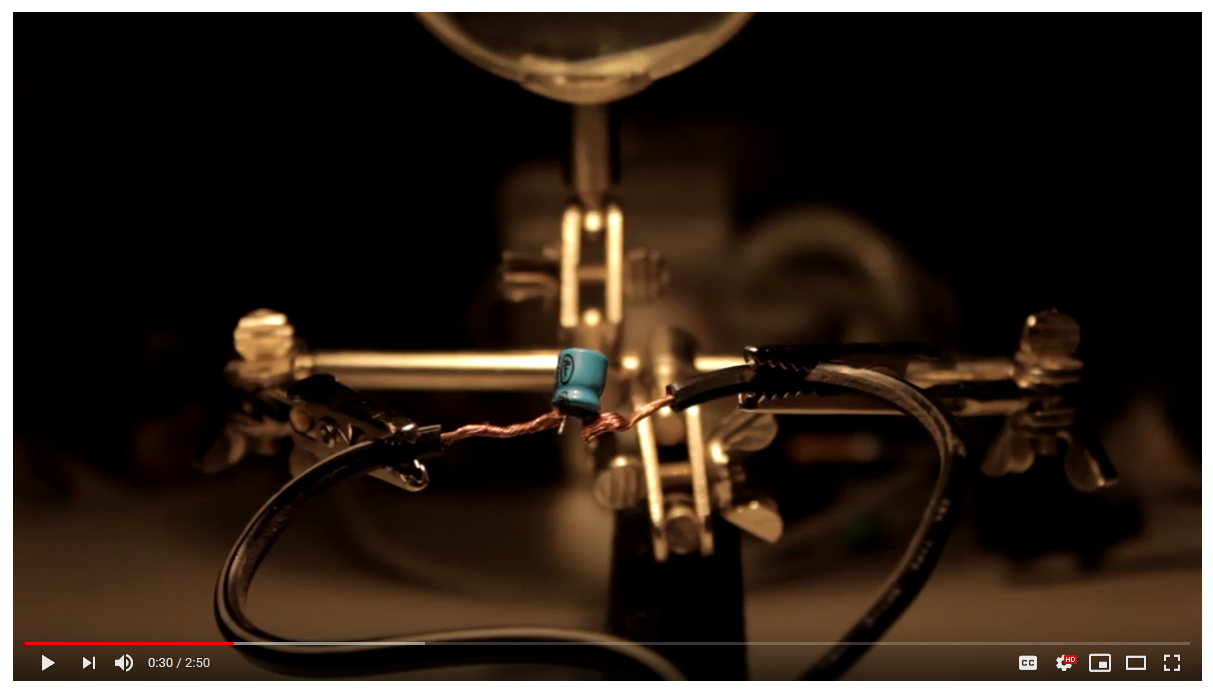
\includegraphics[width=\textwidth]{figures/explosion-condensateur.png}
  \url{https://youtu.be/XBoaBwMRbnk?t=30}
\end{frame}


\begin{frame}{Explosion de condensateurs}

Dans un des cas, on voit un condensateur de \SI{470}{\micro\farad} qui explose.
Supposons qu'il a explosé à une tension de \SI{200}{\volt}. Quelle est la
quantité d'énergie qui peut être relâchée durant cette explosion?

\end{frame}



\begin{frame}{Exercice}

On a deux condensateurs identiques. Le condensateur A porte une charge de
\SI{100}{\micro\farad} et le condensateur B porte une charge de
\SI{50}{\micro\farad}. Quel énoncé est vrai?

\begin{enumerate}[A.]
  \item La capacité du condensateur A est deux fois plus grande que celle du
    condensateur B.
  \item<alert@2> Le champ électrique entre les armatures du condensateur A est
    deux fois plus grand que celui de B.
  \item La différence de potentiel du condensateur A est deux fois plus petite
    que celle de B.
  \item Il y a deux fois plus d'énergie emmagasinée dans le condensateur A que
    le B.
\end{enumerate}

\end{frame}



\begin{frame}{Exercice}

On a deux condensateurs identiques sauf pour le diélectrique. Dans le
condensateur A, le diélectrique est du papier (constante diélectrique de 3).
Dans le condensateur B le diélectrique est du mica (constante diélectrique de
6). Les deux condensateurs portent la même charge. Lequel des énoncés est vrai.

\begin{enumerate}[A.]
  \item La capacité du condensateur A est deux fois plus grande que celle du
    condensateur B.
  \item<alert@2>  Le champ électrique entre les armatures du condensateur A est
    deux fois plus grand que celui de B.
  \item La différence de potentiel du condensateur A est deux fois plus petite
    que celle de B.
  \item Il y a deux fois plus d'énergie emmagasinée dans le condensateur A que
    le B.
\end{enumerate}

\end{frame}


\begin{frame}{Exercice circuit avec condensateur}

On construit le circuit suivant avec une pile de \SI{9}{V}. Le condensateur 1 a
une capacité $C_1 = \SI{45}{\micro\farad}$ et ses armatures sont séparées par
du vide. Les condensateurs 2 et 3 sont construits de la même façon que le
condensateur 1 sauf que l'espace entre leurs armatures est rempli par
du germanium et du papier, respectivement. La constante diélectrique du
germanium est 16 alors que celle du papier est 3.

\begin{center}
\begin{circuitikz}[yscale=0.7]
  % French babel breaks everything... see https://latex.org/forum/viewtopic.php?t=11981
  \shorthandoff{:}\shorthandoff{!}
  \draw (0, 0) to[battery, l=$\SI{9}{\volt}$] (0, 3)
    to[C, l=$C_1$] (2, 3)
    to[C, l=$C_2$] (2, 0)
    to (0, 0);
  \draw (2, 3) to[short] (4, 3)
    to[C, l=$C_3$] (4, 0)
    to (2, 0);
\end{circuitikz}
\end{center}

\begin{enumerate}
  \item Déterminer la capacité équivalente à ces trois condensateurs.
  \item Déterminer la charge accumulée sur la plaque positive du condensateur 2.
  \item Déterminer l'énergie accumulée dans le condensateur 3.
\end{enumerate}

\end{frame}

\end{document}
